
\documentclass[tikz=true]{standalone}
\usepackage[utf8]{inputenc}

\usepackage{tikz}
\usepackage{amsfonts}
\usepackage{amsmath,amssymb}
\usepackage{systeme,mathtools}
\usetikzlibrary{positioning,arrows.meta,quotes}
\usetikzlibrary{shapes,snakes}
\usetikzlibrary{bayesnet}
\tikzset{>=latex}

\begin{document}
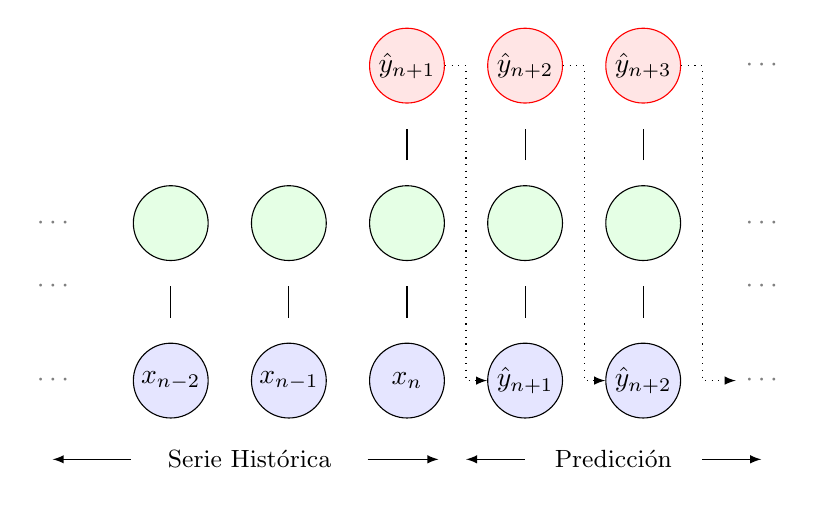
\begin{tikzpicture}

\node[text width=0.4cm] (obs4) at (0,-2) {\color{gray}{$\cdots$}};
\node[circle,draw=black,fill=blue!10,inner sep=0pt,minimum size=0.95cm] (obs2) at (1.5,-2) {$x_{n-2}$};
\node[circle,draw=black,fill=blue!10,inner sep=0pt,minimum size=0.95cm] (obs1) at (3,-2) {$x_{n-1}$};
\node[circle,draw=black,fill=blue!10,inner sep=0pt,minimum size=0.95cm] (obsn) at (4.5,-2) {$x_{n}$};
\node[circle,draw=black,fill=blue!10,inner sep=0pt,minimum size=0.95cm] (obsn1) at (6,-2) {$\hat{y}_{n+1}$};
\node[circle,draw=black,fill=blue!10,inner sep=0pt,minimum size=0.95cm] (obsn2) at (7.5,-2) {$\hat{y}_{n+2}$};
\node[text width=0.4cm] (obsn3) at (9,-2) {\color{gray}{$\cdots$}};

\node[text width=0.4cm] (uu1) at (0,-0.8) {\color{gray}{$\cdots$}};
\draw[] (1.5,-0.8) -- (1.5,-1.2);
\draw[] (3,-0.8) -- (3,-1.2);
\draw[] (4.5,-0.8) -- (4.5,-1.2);
\draw[] (6,-0.8) -- (6,-1.2);
\draw[] (7.5,-0.8) -- (7.5,-1.2);
\node[text width=0.4cm] (uu2) at (9,-0.8) {\color{gray}{$\cdots$}};

\node[text width=0.4cm] (uuu1) at (0,0) {\color{gray}{$\cdots$}};
\node[circle,draw=black,fill=green!10,inner sep=0pt,minimum size=0.95cm] (rnn2) at (1.5,0) {};
\node[circle,draw=black,fill=green!10,inner sep=0pt,minimum size=0.95cm] (rnn3) at (3,0) {};
\node[circle,draw=black,fill=green!10,inner sep=0pt,minimum size=0.95cm] (rnnn) at (4.5,0) {};
\node[circle,draw=black,fill=green!10,inner sep=0pt,minimum size=0.95cm] (rnnn1) at (6,0) {};
\node[circle,draw=black,fill=green!10,inner sep=0pt,minimum size=0.95cm] (rnn2) at (7.5,0) {};
\node[text width=0.4cm] (uuu2) at (9,0) {\color{gray}{$\cdots$}};



\node[circle,draw=red,fill=red!10,inner sep=0pt,minimum size=0.95cm] (out1) at (4.5,2) {$\hat{y}_{n+1}$};
\node[circle,draw=red,fill=red!10,inner sep=0pt,minimum size=0.95cm] (out2) at (6,2) {$\hat{y}_{n+2}$};
\node[circle,draw=red,fill=red!10,inner sep=0pt,minimum size=0.95cm] (out3) at (7.5,2) {$\hat{y}_{n+3}$};
\node[text width=0.4cm] (uuu3) at (9,2) {\color{gray}{$\cdots$}};
\draw[] (4.5,0.8) -- (4.5,1.2);
\draw[] (6,0.8) -- (6,1.2);
\draw[] (7.5,0.8) -- (7.5,1.2);


\node at (2.5,-3) {\small{Serie Histórica}};
\draw[arrows=->] (4,-3)--(4.9,-3);
\draw[arrows=<-] (0,-3)--(1,-3);

\node at (7.12,-3) {\small{Predicción}};
\draw[arrows=->] (8.25,-3)--(9,-3);
\draw[arrows=<-] (5.25,-3)--(6,-3);


\draw[dotted, arrows=->] (out1) -| (5.25,0) |- (obsn1);
\draw[dotted, arrows=->] (out2) -| (6.75,0) |- (obsn2);
\draw[dotted, arrows=->] (out3) -| (8.25,0) |- (obsn3);

\iffalse
\path [draw,->,color=blue!50!green] (obs1) edge [bend left] node [right] {} (obs2);
\node[circle,draw=black,fill=red!10,inner sep=0pt,minimum size=0.85cm] (obs7) at (9,0) {$y_{i,t+2}$};
\node[text width=0.4cm] (obs8) at (10.5,0) {\color{gray}{$\cdots$}};
\path [draw,->,color=blue!50!green] (obs2) edge [bend left] node [right] {} (obs3);
\path [draw,->,color=blue!50!green] (obs3) edge [bend left] node [right] {} (obs4);
\path [draw,->,color=blue!50!green] (obs4) edge [bend left] node [right] {} (obs5);
\path [draw,->,color=red!50!gray] (obs5) edge [bend left] node [right] {} (obs6);
\path [draw,->,color=red!50!gray] (obs6) edge [bend left] node [right] {} (obs7);
\node[text width=0.3cm] (unknown1) at (1.5,-0.0) {\LARGE\color{red!30}{?}};
\node[text width=0.3cm] (unknown1) at (6,-0.0) {\LARGE\color{red!30}{?}};

\node at (3.375,-1) {\small{historical values}};
\draw[arrows=->] (4.85,-1)--(6.75,-1);
\draw[arrows=<-] (0,-1)--(1.9,-1);
\node at (8.625,-1) {\small{near-future values}};
\draw[arrows=->] (10.2,-1)--(10.5,-1);
\draw[arrows=<-] (6.75,-1)--(7.05,-1);
\fi
\end{tikzpicture}
\end{document}
